\chapter{Background}
\label{ch:Background}
In this chapter we define the necessary background for understanding PGExplainer as well as the follow-up work regarding its application on SAT.

\section{Deep learning}
What is machine learning? What is Deep learning? \\
Principle behind neural networks: Layers, gradients, gradient descent?, backprop...
\subsection{MLP}

\subsection{Batchnorm, LayerNorm, ...}


\section{Graph Theory}
These definitions will loosely follow Brachman et al.\cite{}. A graph is a data structure consisting of a set of nodes that are connected via edges, modeling objects and their relationships. It can be represented as $G=(V,E)$ with $V=\{v_1,v_2...v_n\}$ being the set of $n$ nodes, and $E \in V \times V$ the set of edges. An edge $e=(u,v)$ connects nodes $u$ and $v$, making them neighbours. Edges are either directed or undirected and lead to directed or undirected graphs if exclusively present. The degree of a node $v$ is the number of edges connected to $v$ and denoted by $d(v)$. $G$ can be described by an adjacency matrix $A \in \mathbb{R}^{n \times n}$, where
$$A_{ij}=\begin{cases}
    1 & \text{if } \{v_i,v_j\}\in E \text{ and } i \neq j, \\
    0 & \text{otherwise.}
\end{cases}$$
If $G$ is an undirected Graph the adjacency matrix will be symmetrical. We adopt the conventions from Diestel\cite{Diestel2017} to refer to the node and edge set of any graph $G$ with $V(G)$ and $E(G)$, regardless of the actual names of the sets, as well as a referring to $G$ with node set $V$ as $G$ on $V$. $G$ is called a subgraph of another graph $G'=(V',E')$ if $V(G) \subseteq V(G')$ and $E(G) \subseteq E(G')$. This is denoted as $H \subseteq G$. The number of nodes in a graph $|V|$ is its order and the number of edges $|E|$ is its size.
We additionally define bipartite graphs according to Asratian et al.\cite{asratian1998}: A graph $G$ is bipartite if the set of nodes $V$ can be partitioned into two sets $V_1$ and $V_2$ so that no two nodes from the same set are adjacent. The sets $V_1$ and $V_2$ are called colour classes and $(V_1, V_2)$ is a bipartition of $G$. This means that if a graph is bipartite all nodes in $V$ can be coloured by at most two colours so that no two adjacent nodes share the same colour.\\
TODO: EDGE WEIGHTS, K-hop/computational graph?
\begin{figure}[h]
    \centering
    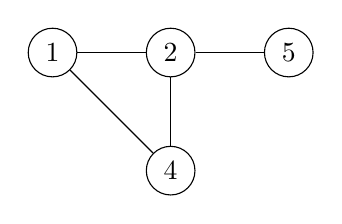
\begin{tikzpicture}[node distance=1.5cm, every node/.style={draw, circle}]
        % Define Nodes
        \node (1) {1};
        \node (2) [right of=1] {2};
        \node (4) [below of=2] {4};
        \node (5) [right of=2] {5};
        
        % Draw Edges
        \draw (1) -- (2);
        \draw (2) -- (4);
        \draw (1) -- (4);
        \draw (2) -- (5);
    \end{tikzpicture}
    \caption{A simple undirected graph $G$ with $V=\{1,...,5\}$ and $E=\{\{1,2\},\{2,4\},\{1,4\},\{2,5\}\}$}
    \label{fig:graph-example}
\end{figure}

\subsection{Graph generation/Graph Generative Model/Random Graphs}
Erdos-Renyi model first model of random graphs, but slightly different from Gilbert. \bigskip

TODO: WRONG! (Independent experiments with same probability!) Gilbert\cite{} describes the process of generating a random graph G of order N by assigning independent probabilities $p$ to each potential edge between two nodes in $V(G)$ to exist in $E(G)$(, effectively drawing from a Bernoulli distribution). \\
A random graph is further described by Diestel\cite{} as follows. Let $V = \{0,...,n-1\}$ be a fixed set of $n$ elements. Our goal is to define the set $\mathcal{G}$ of all graphs on $V$ as a probability space, which allows us to ask whether a Graph $G \in \mathcal{G}$ has a certain property. To generate our random graph we then decide from some random experiment whether $e$ shall be an edge of $G$ for each potential $e \in [V]^2$. The probability of success - accepting $e$ as edge in $G$ - is defined as $p \in [0,1]$ for each experiment. TODO: Rewrite the accepting part. This leads to the probability of $G$ being a particualar graph $G_0$ on $V$ with e.g. $m$ edges being equal to $p^m q^{\binom{n}{2}-m}$ with $q:=1-p$. It follows our desired probability space $\mathcal{G}=(n,p)$ as the product space
$$\Omega := \prod_{e \in [V]^2} \Omega_e$$ with $\Omega_e := \{0_e,1_e\}$, $\mathbb{P}_e(\{1_e\}) := p$ and $\mathbb{P}_e(\{0_e\}) := q$.
$$E(G) = \{e | \omega(e) = 1_e\}$$
G is called a random graph on V with egde probability p. \bigskip

TODO: Define $[V]^2$ as the set of all 2-elements subsets of V? or rewrite as e in E x E \\
INSTEAD: Gilberts idea also assigns the same probability across all edges, so probably best to explain the general idea as presented in Diestel. Then explain the difference in PGE? PGEs appraoch mainly inspired by probabilistic graphical model/bayesian networks. Gilbert model mainly baseline for probabilistic graphs. PGExplainer mainly inspired by Gilbert, but "required" concept is PGM.

\section{Information Theory}
To fully understand the learning objective of PGExplainer it is necessary to define the concepts of entropy and mutual information. We follow the definitions by Cover et al.\cite{Cover2005}[p.13].

\subsection{Entropy}
Entropy is used to describe the uncertainty of a random variable. Let $X$ be a discrete random variable with alphabet $\mathcal{X}$ and probability mass function $p(x)=Pr\{X=x\}$ for $x\in X$.
The entropy $H(X)$, also written as $H(p)$ is defined as
\begin{equation}
    H(X) = -\sum_{x \in \mathcal{X}} p(x) \log p(x).
\end{equation}
The log is to the base 2 and entropy is measured in bits. TODO: DEFINE EDGE CASES log 0 TODO: TOO MUTCH + SOURCE? A simple example is tossing two coins: There are four possible outcomes $\mathcal{X}=\{00,10,01,11\}$, each with a probability $p=0,25$. The resulting entropy $H(X)=2$ represents that two bits of information can be stored this way. \bigskip

TODO: NOT USED IN PGE, ONLY FOR DEFINITION OF COND. ENT. IF KEPT, DIFFER MORE CLEARLY FROM CROSS? \\
Analogously we define the joint entropy $H(X,Y)$ of a pair of discrete random variables $(X,Y)$ with a joint distribution $p(x,y)$ as follows:
\begin{equation}
    H(X,Y)=-\sum_{x \in \mathcal{X}} \sum_{y \in \mathcal{Y}} p(x,y) \log p(x,y).
\end{equation}
TODO: REWRITE! MAYBE NOT NEEDED AS NOT "USED" IN PGE? \\
The conditional entropy of $Y$ given $X$ is defined as the expected value of the entropies of the conditional distributions, averaged over the conditioning random variable. If $(X,Y) \sim p(x,y)$ the conditional entropy is defined as
\begin{align}
    H(Y|X)&= -\sum_{x \in \mathcal{X}} p(x) H(Y|X=x) \\
    &= - \sum_{x \in \mathcal{X}} \sum_{y \in \mathcal{Y}}p(x,y) \log p(y|x) \\
    &= -E \log p(Y|X) \text{ with E = Expectation}.
\end{align}

Elements of Information Theory: equation 2.26 describes KL distance/relative entropy \bigskip

TODO: KL distance or relative entropy with probability mass functions $p(x), q(x)$:
\begin{equation}
    D_{KL}(p||q) = \sum_{x \in \mathcal{X}} p(x)\log \frac{p(x)}{q(x)}
\end{equation}

Cross entropy by Goodfellow et al.\cite{Goodfellow-et-al-2016}[p.75] assumes probability distributions P, Q:
\begin{equation}
    H(P,Q)= -\mathbb{E}_{x\sim P}\log Q(x)
\end{equation}
Closely related to KL divergence and can therefore also be expressed as:
\begin{equation}
    H(P,Q) = H(P) + D_{KL}(P||Q)
\end{equation}

We derive for the discrete case with mass probability functions p, q with the same support $\mathcal{X}$ (TODO: NOT NEEDED? for random Variables X, Y):
\begin{align}
    H(p,q) = H(p) + D_{KL}(p||q) &= -\sum_{x \in \mathcal{X}} p(x) \log p(x) + \sum_{x \in \mathcal{X}} p(x)\log \frac{p(x)}{q(x)} \\
    &= -\sum_{x \in \mathcal{X}} p(x) \log p(x) + \sum_{x \in \mathcal{X}} p(x) \log p(x) -\sum_{x \in \mathcal{X}} p(x) \log q(x) \\
    &= -\sum_{x \in \mathcal{X}} p(x) \log q(x)
\end{align}

The approach in PGExplainer is a common approach in ML for simplifying objectives? FIND LITERATURE THAT EXPLAINS APPROXIMATION OF COND. ENTROPY WITH CROSS ENTROPY \bigskip

"We can modify the conditional entropy objective in Equation 4 with a cross entropy objective between the label class and the model prediction" (GNNExplainer)

\subsection{Mutual Information}
Another closely related concept is mutual information (see Cover et al.\cite{Cover2005}[p.19]). It measures the amount of information that one random variable contains about another or the reduction in uncertainty of said variable due to knowing the other.
Let $X$ and $Y$ be two random variables with the joint probability mass function $p(x,y)$ and marginal probability mass functions $p(x)$ and $p(y)$. Mutual information $I(X;Y)$ is the relative entropy between the joint distribution and product distribution $p(x)p(y)$: 
\begin{align}
    I(X;Y)&=\sum_{x \in \mathcal{X}}\sum_{y \in \mathcal{Y}} p(x,y)\log \frac{p(x,y)}{p(x)p(y)} \\
    &= H(X) - H(X|Y)
\end{align}

\subsection{Monte Carlo Sampling}
Goodfellow et al.\cite{Goodfellow-et-al-2016}[p.590] TODO: EXPLANATION \\
Let 
\begin{equation}
    s = \sum_x p(x)f(x)=E_p[f(x)]
\end{equation}
be the sum to estimate with $p$ being a probability distribution over a random variable $x$. Then $s$ can be approximated by drawing $n$ samples from $p$ and constructing the empirical average 
\begin{equation}
    \hat{s}_n=\frac{1}{n}\sum_{i=1}^n f(x^{(i)}).
\end{equation}

\section{Graph Neural Networks}

The following definitions will loosely follow book/... (reference).
JEDE Variable einmal erklärt! Einheitliche Variablen aus meiner Sicht

Graph Neural Networks(GNNs)\cite{4700287} are a deep learning-based approach that operates on graphs, a data structure consisting of nodes and edges, representing objects and their relationships. Due to their unique non-Euclidean property, they find usage in classification, link prediction, and clustering tasks. Their high interpretability and strong performance have led to GNNs becoming a commonly employed method in graph analysis. They combine the key features of convolutional neural networks\cite{726791}, such as local connection, shared weights, and multi-layer usage, with the concept of graph embeddings\cite{cai2018comprehensive} to leverage the power of feature extraction and representation as low-dimensional vectors for graphs\cite{Liu2020}. \\
- difference node task, graph tasks (Scarselli) \\
- data preprocessed: mapping to simpler representation
- encode graph structure/topology to keep structural information
- directed/undirected?
- ...



\subsection{Convolutional Graph Neural Networks}
Explain? Used in architecture of downstream task, only slightly relevant

\section{Perturbation-based Explainability in GNNs}
Explainability methods in the context of deep learning and further GNNs \\
Different approaches, further into perturbation based... \bigskip

- Common metric to measure accuracy of explanation methods in comparison to ground truth is ROC-AUC score? (Explain/name first in results?)
- Other metric includes fidelity, results of taxonomy propose only using PGExplainer for Node Classification as it achieves low fidelity on Graph tasks

\section{Boolean Satisfiability Problem}
We define the Boolean Satisfiability Problem (SAT) according to Guo et al.\cite{guo2023machine}[p.641]: \\
A Boolean formula is constructed from Boolean variables, that only evaluate to True (1) or False (0), and the three logic operators conjunction ($\wedge$), disjunction ($\vee$) and negation ($\neg$). SAT aims to evaluate whether there exists a variable assignment for a formula constructed of said parts so that it evaluates to True. If so, the formula is said to be satisfiable or unsatisfiable otherwise. Every propositional formula can be converted into an equivalent formula in conjunctive normal form (CNF), which consists of a conjunction of one or more clauses. These clauses must contain only disjunctions of at least one literal (a variable or its negation). In this work we consider only formulas in CNF, as NeuroSAT\cite{} assumes SAT problems to be in CNF. An example of a satisfiable formula in CNF over the set of variables $V=\{x_1,x_2\}$ is 
$$\psi(V) = (x_1) \land (\neg x_1 \lor x_2) \land (\neg x_2 \lor x_2)$$
with satisfying assignment $A:\{x_1 \mapsto 1, x_2 \mapsto 1\}$. Furthermore, SAT is $NP$-complete, meaning that if there exists a deterministic algorithm able to solve SAT in polynomial time, then such an algorithm exists for every $NP$ problem.

\subsection{Representation as Bipartite Graph}
From Guo: 4 types of graph representations for CNF formulae: LCG, LIG, VCG, VIG.
"LCG is a bipartite graph with literals on one side and clauses on the other side, with edges connecting literals to the clauses where they occur."
Representation of SAT in context of NeuroSAT: literal-clause graph (LCG). Messages are passed between clauses and literals, as well as literals and their complement. 1. Clause receives from neighboring literals 2. Literals receive from clauses and complement. \\
Formal definition as incident graph?

TODO: TOO BIG
\begin{figure}[h]
    \centering
    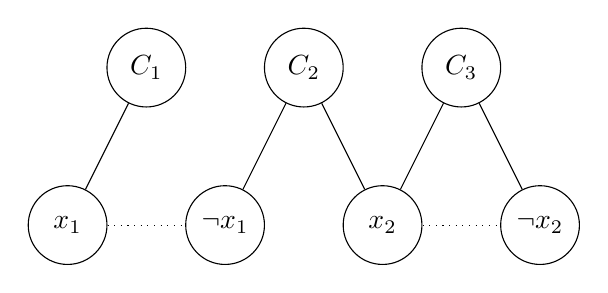
\begin{tikzpicture}[
        every node/.style={draw, circle, minimum size=1cm},
        node distance=1.5cm,
        scale=0.8,
    ]
        % Define Literal Nodes
        \node (x1) at (0, 0) {\(x_1\)};
        \node (notx1) at (2.5, 0) {\(\neg x_1\)};
        \node (x2) at (5, 0) {\(x_2\)};
        \node (notx2) at (7.5, 0) {\(\neg x_2\)};
        
        % Define Clause Nodes (one level above literals)
        \node[circle, draw] (C1) at (1.25, 2.5) {\(C_1\)};
        \node[circle, draw] (C2) at (3.75, 2.5) {\(C_2\)};
        \node[circle, draw] (C3) at (6.25, 2.5) {\(C_3\)};
        
        % Draw Edges (Literal → Clause)
        \draw (x1) -- (C1);
        \draw (notx1) -- (C2);
        \draw (x2) -- (C2);
        \draw (notx2) -- (C3);
        \draw (x2) -- (C3);
        
        % Draw Dotted Edges between each literal and its co mplement
        \draw[dotted] (x1) -- (notx1);
        \draw[dotted] (x2) -- (notx2);
    \end{tikzpicture}
    \caption{LCG representation for $\psi(V)$}
    \label{fig:lcg-sat}
\end{figure}

\subsection{Incidence/Levi graph?}
Defined in ALYAHYA et al. Concrete graphical representation of SAT? Type of bipartite graph.
Defines edges via edge weight function! PART OF GRAPH THEORY \\
Definition in Cimatti et al. : For clause $c$ we use $lit(c)$ and $var(c)$ to reference the set of literals and variables in $c$ respectively. "$For a CNF formula F we write
cla(F) for its set of clauses, lit(F)= c \in cla(F) lit(c) for its set of literals, and
var(F)= c \in cla(F) var(c) for its set of variables.$"  Incidence graph of $\psi$ is the bipartite graph $inc(\psi) = (V,E)$ with $V=lit(\psi) \cup cla(\psi)$. Additionally for literal $x \in lit(\psi)$ and clause $c \in cla(\psi)$ we define $xc \in E$ if $x \in var(c)$.

ALTERNATIVE: Describe levi graph shortly. Then define convention for our definitions of sat and the respective incidence graph that follows?

\subsection{UNSAT Cores}
Instances of SAT are commonly analyzed as graphs

\subsection{Backdoors}
Definition in Cimatti et al.

\section{NeuroSAT}
